\documentclass[12pt,  english, makeidx, a4paper, titlepage, oneside]{article}
\usepackage[english]{babel}
\usepackage[applemac]{inputenc}
\usepackage{fancyhdr}
\usepackage{makeidx}
\usepackage{titlesec}
\usepackage{listings} 
\newenvironment{listato}{\footnotesize}
                        {\normalsize }
\textwidth 19cm
\textheight 23cm
\topmargin -1.5cm
\oddsidemargin -1.5cm
\linespread{1.1}

\pagestyle{fancy}
\lhead{}
\chead{NAND/AND Modules}
\lfoot{}
\cfoot{}
\rfoot{}
\rhead{\thepage}

\usepackage{graphicx}
\usepackage{amsmath}
\usepackage{amsfonts}
\usepackage{amsthm}
\usepackage{amssymb}
\usepackage{epstopdf}

\titleformat{\chapter}[display]
{\normalfont\Large\filcenter\sffamily}
{\titlerule[0.5pt]%
\vspace{1pt}
\titlerule
\vspace{1pc}
\LARGE\MakeUppercase{\chaptertitlename} \thechapter
}
{1pc}
{\titlerule
\vspace{1pc}
\Huge}

\makeindex


\begin{document}
	\begin{titlepage}
		\vspace{1cm}
		\centerline{
			
\includegraphics[width=2cm]{./img/logopoli.eps}}  
		\centerline{\LARGE Politecnico di Torino}
		\bigskip
		\vspace{3cm}
		\centerline{\LARGE TAMTAMS Web}
		\vspace{0.5cm}
		\centerline{\Large Integrated System Technology}
		\vspace{3cm}
		\centerline{\huge NAND/AND MODULES:}
		\vspace{0.7cm}
		\centerline{\Large\sf Delay\_Pow\_nand2\_cmos, Delay\_Pow\_nand3\_cmos, Delay\_Pow\_nand4\_cmos}
		\vspace{0.3cm}
		\centerline{\Large\sf Delay\_Pow\_nor2\_cmos, Delay\_Pow\_nor3\_cmos, Delay\_Pow\_nor4\_cmos}
		\bigskip
		\vspace{5cm}
\centerline{\Large Simone Aiassa\\Alberto Cassisa\\Giovanni Fazio}
\vspace{1cm}
\centerline{\Large \today}
\end{titlepage}

\tableofcontents

\newpage

\lstset{language=Matlab}

\newpage


\section{Introduction}

% % % % % % % % % % % % % %da fare % % % % %

Analysis and parameters estimation in terms of power and delay of different single logic gates.
To do that \textit{NAND2, NAND3, NAND4}  and \textit{NOR2, NOR3, NOR4} logic gates implemented in \textit{CMOS-logic} are analysed.  \\
This \textit{OCTAVE} files are implemented for \textit{TAMTAMS}: 
\begin{itemize}
\item \textbf{Delay\_Pow\_nand2\_cmos.m}: CMOS-logic 2-inputs NAND;
\item \textbf{Delay\_Pow\_nand3\_cmos.m}: CMOS-logic 3-inputs NAND;
\item \textbf{Delay\_Pow\_nand4\_cmos.m}: CMOS-logic 4-inputs NAND;
\item \textbf{Delay\_Pow\_nor2\_cmos.m}: CMOS-logic 2-inputs NOR;
\item \textbf{Delay\_Pow\_nor3\_cmos.m}: CMOS-logic 3-inputs NOR;
\item \textbf{Delay\_Pow\_nor4\_cmos.m}: CMOS-logic 4-inputs NOR;
\end{itemize}

where the following parameters are estimated:

\begin{itemize}
\item \textbf{Delay\_nand\_and}: input to output delay;
\item \textbf{Pnand\_and\_dyn}: dynamic power;
\item \textbf{Pnand\_and}: static power;
\end{itemize}
 
\newpage 
\section{Logic Implementation}

\label{section:logicimplementation}
The different logic gates involved into the analysis are represented in form of schematic.\\
The dimension of the transistor are forced in order to have a resistance (and an $I_{on}$) equal to the inverter of minimal dimension.\\
In figure \ref{fig:CMOSGRID} is possible to see the reference schematic for the \textit{CMOS} logic. The structure is the most known one based on a pull-up and a pull-down structure.\\

\begin{figure}[htbp]
\begin{center}
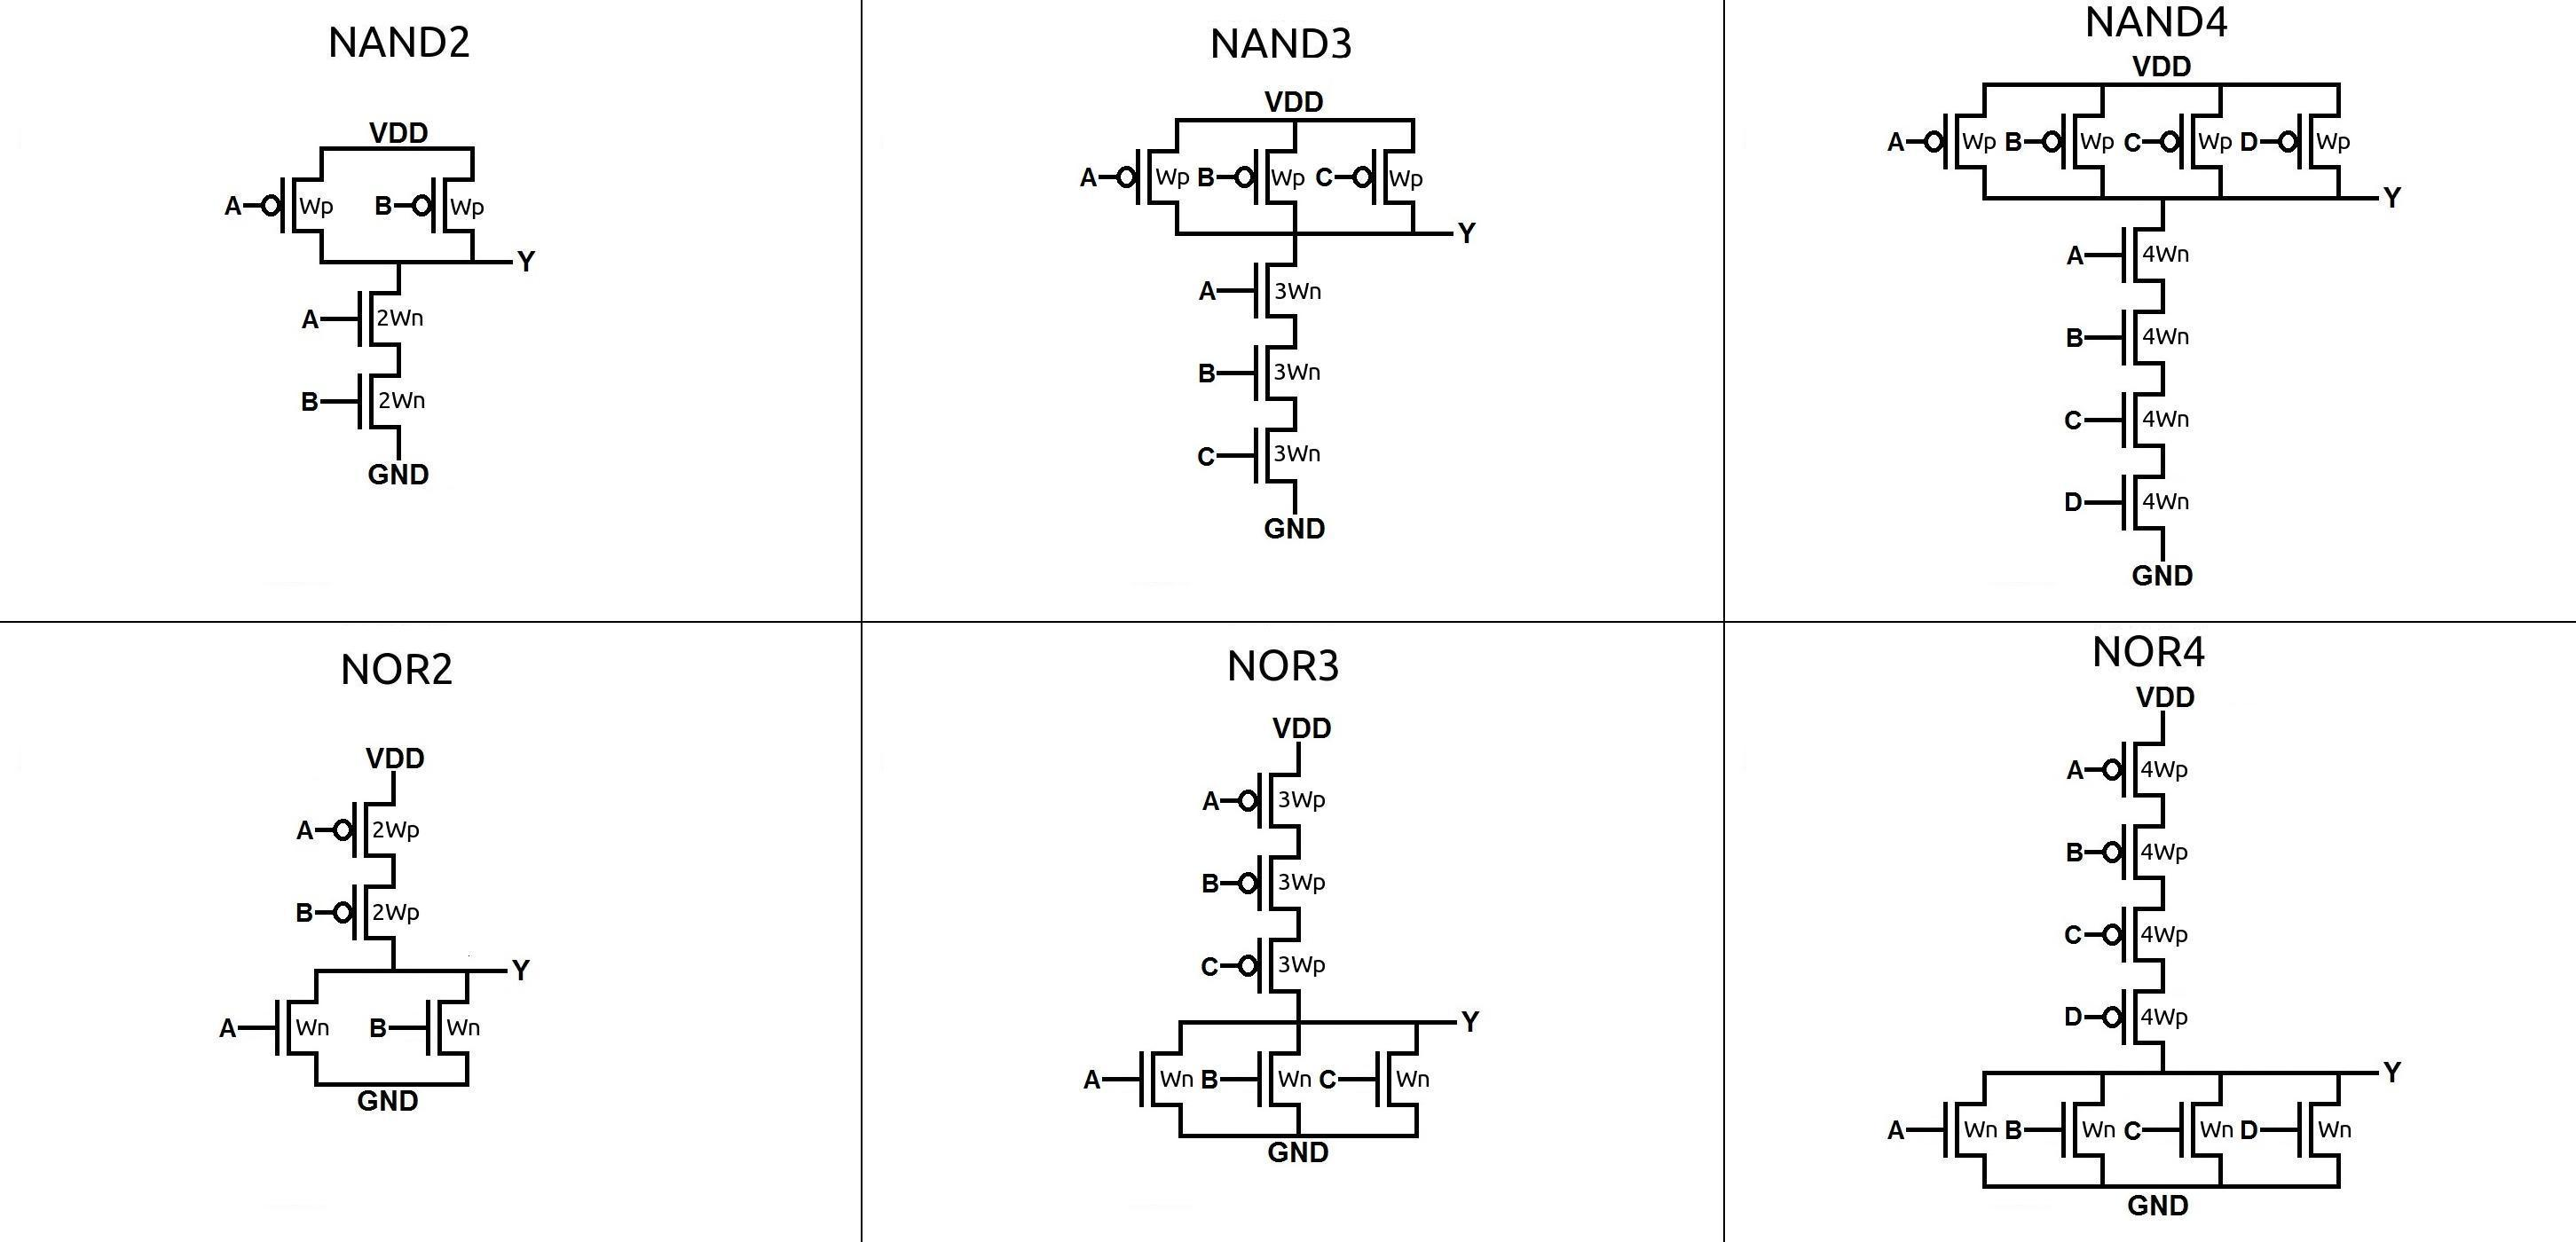
\includegraphics[width=19cm]{img/CMOS_GRID.jpg}
\caption{CMOS schemes}
\label{fig:CMOSGRID}
\end{center}
\end{figure}
\newpage




\section{Delay}


\subsection{Theoretical Analysis}
\label{captech*}
The delay analysis of the different gates is implemented exploiting the \textit{Elmore} Delay model, taking into account that it is an optimistic model. Moreover it could be used to easily compare different technological implementation.\\
Necessary technological parameters in order to evaluate the delay are reported below.\\
The analysis is done on gate with a load made of a minimum inverter or multiple of it. Is possible compute input capacitance of \textit{n-MOS} and \textit{p-MOS} transistors per unit length:
\begin{eqnarray}
C_{in_N}=C_{OX}+C_{overlapN} \quad [pF/\mu m]\\
C_{in_P}=C_{OX}+C_{overlapP} \quad [pF/\mu m]
\end{eqnarray}
where the two overlap capacitances are due to the overlap size between the gate and drain/source areas:
\begin{eqnarray}
C_{overlapN}=10^6 \cdot C_{GDOn} \quad [pF/\mu m]\\
C_{overlapP}=10^6 \cdot C_{GDOp} \quad [pF/\mu m]
\end{eqnarray}
The junction capacitances between source and drain are:
\begin{eqnarray}
C_{jN}=C_{bottomN} + C_{sidewallN} \quad [pF/\mu m]\\
C_{jP}=C_{bottomP} + C_{sidewallP} \quad [pF/\mu m]
\end{eqnarray}
$C_{bottom}$ is the capacitance due to the area of the pool of the source/drain and $C_{sidewall}$ is the one due to the edge of the same pool.
\begin{eqnarray}
C_{bottomN}=C_{j0_N} \cdot \Bigl(1+ \frac{V_{DD}}{2 \cdot P_{bN}} \Bigr)^{-M_{jN}} \cdot 2.5 \cdot L_{drawn} \quad [pF/\mu m]\\
C_{bottomP}=C_{j0_P} \cdot \Bigl(1+ \frac{V_{DD}}{2 \cdot P_{bP}} \Bigr)^{-M_{jP}} \cdot 2.5 \cdot L_{drawn} \quad [pF/\mu m]\\
C_{sidewallN}=10^6 \cdot C_{sw_N} \cdot \Bigl(1+ \frac{V_{DD}}{2 \cdot P_{bswN}} \Bigr)^{-M_{jswN}} \quad [pF/\mu m]\\
C_{sidewallP}=10^6 \cdot C_{sw_P} \cdot \Bigl(1+ \frac{V_{DD}}{2 \cdot P_{bswP}} \Bigr)^{-M_{jswP}} \quad [pF/\mu m]
\end{eqnarray}
Moreover for the estimation of parasitic capacitances $C_{jN}$ and $C_{jP}$, it is necessary to evaluate the perimeter.
\begin{eqnarray}
\text{perim}_N=2 \cdot \text{lungh\_diff} + W_N [\mu m]\\
\text{perim}_P=2 \cdot \text{lungh\_diff} + W_P [\mu m]
\end{eqnarray}
We consider only one side for the $W$, because the internal one does not touch a conductor, but just a spatial charge. \\Therefore $C_{jN}$ and $C_{jP}$ are:
\begin{eqnarray}
C_{jN}=C_{bottomN} \cdot W_N + C_{sidewallN} \cdot \text{perim}_N \quad [pF]\\
C_{jP}=C_{bottomP} \cdot W_P + C_{sidewallP} \cdot \text{perim}_P \quad [pF]
\end{eqnarray}
\\ Now we have to evaluate the equivalent resistance of the \textit{MOS} that contributes in the delay calculation:
\begin{equation}
R_n=\frac{1}{\mu_n \cdot C_{OX} \cdot \frac{W_N}{L_{eff}}\cdot (V_{DD}-V_{tn})} \quad [\Omega]
\end{equation}\\
\begin{equation}
R_p=\frac{1}{\mu_p \cdot C_{OX} \cdot \frac{W_P}{L_{eff}}\cdot (V_{DD}-V_{tp})} \quad [\Omega]
\end{equation}\\
Another parameters used in our analysis is \textit{h}. It's simply the multiplier of the number of inverter linked in output, the parametrized fan-out.

\subsection{Delay calculation}
In figure:\ref{fig:nand_2_cmos} the \textit{Elmore} model of \textit{NAND2-CMOS} gate is shown. The computation are made by summing partial product between parasitic capacitance and resistance. To compute the delay of all gates in analysis the same model it's applied.
\begin{figure}[htbp]
	\begin{center}
		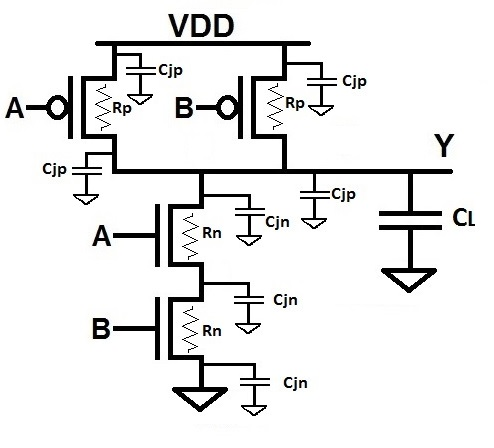
\includegraphics[width=0.5\textwidth]{img/NAND2_StaticLogic_delay.jpg}
		\caption{CMOS-NAND2 Elmore Model}
		\label{fig:nand_2_cmos}
	\end{center}
\end{figure}\\
Obviously there are different delay depending on the inputs combinations, we take in account the worst case that produce the maximum delay for the gate.
For example is easy to see that the worst case for the rise time in the \textit{NAND2} is when only one of the inputs it's low, because in case of all input in \textit{low-state} the resistance is halved. While for the fall time there is only one case. All these reasoning are specular in the \textit{NOR} gates.
\\
\begin{itemize}
	\item \textbf{NAND2-CMOS}
	\begin{equation}
	tr_{cnand2}= R_p \cdot ( C_{jp} + C_{jp} + C_{jn} + h\cdot C_L ) = R_p\cdot (2\cdot C_{jp} + C_{jn} + h \cdot C_L )
	\end{equation}
	\begin{equation}
	tf_{cnand2}= R_n \cdot (  C_{jn} + C_{jn} +C_{jp} + C_{jp} + h \cdot C_L ) +  R_n \cdot (  C_{jn} +C_{jp} + C_{jp} +h \cdot C_L ) =  R_n \cdot ( 3\cdot C_{jn} + 4 \cdot C_{jp} + 2\cdot h \cdot C_L )
	\end{equation}
	\item\textbf{NAND3-CMOS}
	\begin{equation}
	tr_{cnand3}= R_p\cdot (3\cdot C_{jp} + C_{jn} + h \cdot C_L )
	\end{equation}
	\begin{equation}
	tf_{cnand3}=   R_n \cdot ( 6\cdot C_{jn} + 9 \cdot C_{jp} + 3\cdot h \cdot C_L )
	\end{equation}
	\item\textbf{NAND4-CMOS}
	\begin{equation}
	tr_{cnand4}= R_p\cdot (4\cdot C_{jp} + C_{jn} + h \cdot C_L )
	\end{equation}
	\begin{equation}
	tf_{cnand4}=   R_n \cdot ( 10\cdot C_{jn} + 16 \cdot C_{jp} + 4\cdot h \cdot C_L )
	\end{equation}
	\item\textbf{NOR2-CMOS}
	\begin{equation}
	tr_{cnor2}= R_p \cdot (  C_{jn} + C_{jn} +C_{jp} + C_{jp} + h \cdot C_L ) +  R_p \cdot (  C_{jn} +C_{jp} + C_{jp} + h \cdot C_L ) =  R_p \cdot ( 3\cdot C_{jn} + 4 \cdot C_{jp} + 2\cdot h \cdot C_L )
	\end{equation}
	\begin{equation}
	tf_{cnor2}= R_n \cdot ( C_{jn} + C_{jn} + C_{jp} + h \cdot C_L ) = R_p\cdot (2\cdot C_{jn} + C_{jp} + h \cdot C_L )
	\end{equation}
	
	\item\textbf{NOR3-CMOS}
	\begin{equation}
	tr_{cnor3}= R_p \cdot ( 6\cdot C_{jp} + 9 \cdot C_{jn} + 3\cdot h \cdot C_L )
	\end{equation}
	\begin{equation}
	tf_{cnor3}= R_n \cdot(3\cdot C_{jn} + C_{jp} + h \cdot C_L )
	\end{equation}
	\item\textbf{NOR4-CMOS}
	\begin{equation}
	tr_{cnor4}= R_p \cdot ( 10\cdot C_{jp} + 16 \cdot C_{jn} + 4\cdot h \cdot C_L )
	\end{equation}
	\begin{equation}
	tf_{cnor4}= R_n \cdot(4\cdot C_{jn} + C_{jp} + h \cdot C_L )
	\end{equation}
\end{itemize}




\newpage


\section{Dynamic Power}
\subsection{Theoretical Analysis}
The dynamic power can be evaluated through the following:
\begin{equation}
P_{dynamic}=\frac{1}{2} \cdot f \cdot C \cdot \alpha \cdot V_{DD}^{2} \quad [W]
\end{equation}
Where $\alpha$ is the switching activity, f the frequency and C the  total capacitance.\\
This analysis was made imposing two assumption in order to get simplified expression to easily make consideration on the technological behaviour of described gates:
\begin{itemize}
	\item The input probability is always considered as $\frac{1}{2}$;
	\item The computation of the switching activity for every single node is based on a \textit{probabilistic model} (shown in detail later). 
\end{itemize}   
All the necessary technological parameters involved into this analysis are detailed in \ref{captech*}.
\subsection{Dynamic power calculation}
For demonstrative purpose a procedure to calculate the dynamic power of the \textit{NAND2-CMOS} gate is reported.\\
In Figure \ref{NAND2_StaticLogic} the scheme of the \textit{NAND2} gate is shown.
\begin{figure}[htbp]
	\begin{center}
		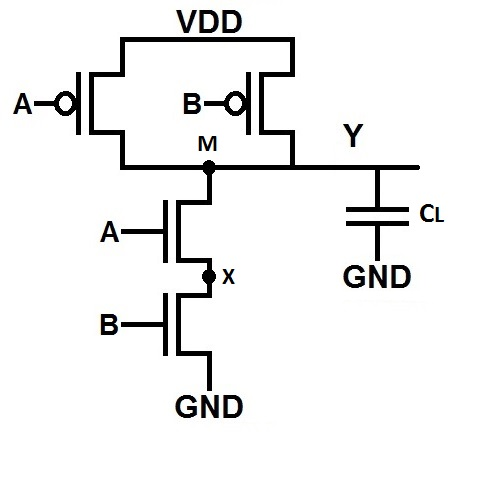
\includegraphics[width=0.5\textwidth]{img/NAND2_StaticLogic_PotDyn}
		\caption{CMOS 2-input NAND architecture}
		\label{NAND2_StaticLogic}
	\end{center}
\end{figure}


\begin{equation}
C \cdot \alpha = C_{IN} \cdot (\alpha_A + \alpha_B)+ C_M \cdot \alpha_M+C_X \cdot \alpha_X
\end{equation}
The considered capacitances are the following:
\begin{itemize}
	\item $C_{IN}$ is the input capacitance associate at only one input:
	\begin{equation}
	\begin{split}& 
	C_{IN}= C_{OX} \cdot 2W_N \cdot L_{eff} + C_{OX} \cdot W_P \cdot L_{eff} + 2C_{overlapN}+ 2C_{overlapP}=\\&
	 = 2C_{OXN} + C_{OXP} + 2C_{overlapN}+ 2C_{overlapP} \quad [pF]
	\end{split}
	\end{equation}
	
	\item $C_{M}$ is the output capacitance:
	\begin{equation}
	C_{M}=2C_{jN} + 2C_{jP}+C_L \quad [pF]
	\end{equation}
	$C_{jP}$ is multiplied by 2 because we have different pools for the two drains and $C_{jN}$ is also multiplied by 2 because the \textit{n-MOS} have dimension $2W_N$
	.
	\item $C_{X}$ is the internal capacitance between the two \textit{n-MOS} transistors in the pull-down network, supposing that source and drain are common for the two \textit{n-MOS}:
	\begin{equation}
	C_{X}=2C_{jN} \quad [pF]
	\end{equation}	
\end{itemize}
Regarding the switching activity it can be computed in the following way if the \textit{probabilistic model} is considered :
\begin{equation}
	\alpha=2P(1-P)
\end{equation}
Where P is the probability that the generic node is at \textit{one}.
Supposing that the probability of each input to be at \textit{one} is $\frac{1}{2}$ we get:
\begin{equation}
\alpha_A = \alpha_B = \frac{1}{2}
\end{equation}
For the node M:
\begin{equation}
P_M = 1-P_A \cdot P_B \rightarrow \alpha_M= \frac{3}{8}
\end{equation}
For the internal node X, the probability is given by:
\begin{equation}
P_X = P_A(1-P_B) \rightarrow \alpha_X= \frac{1}{2}
\end{equation}
Summing up the final expression is the following:
\begin{equation}
	C \cdot \alpha =  2C_{OXN} + C_{OXP} + 2C_{overlapN}+ 2C_{overlapP} +\frac{3}{8} \cdot (2C_{jN} + 2C_{jP}+C_L) +\frac{1}{2} \cdot 2C_{jN}
\end{equation}
The other logic gates are analysed in similar way.\\
Here are reported just the final expression for $ C \cdot \alpha $ in those cases:
\begin{itemize}
	\item  \textbf{NAND3-CMOS}: 
	\begin{equation}
	C \cdot \alpha_{CNAND3} = \frac{3}{2} \cdot (3C_{OXN} + C_{OXP} + 2C_{overlapN}+ 2C_{overlapP} )+\frac{7}{32} \cdot (3C_{jN} + 3C_{jP}+C_L) +\frac{19}{32} \cdot 3C_{jN} 
	\end{equation}
	\item  \textbf{NAND4-CMOS}:
		\begin{equation}
	C \cdot \alpha_{CNAND4} = 2 \cdot (4C_{OXN} + C_{OXP} + 2C_{overlapN}+ 2C_{overlapP} )+\frac{11}{94} \cdot (4C_{jN} + 4C_{jP}+C_L) +\frac{5}{9} \cdot 4C_{jN}
		\end{equation}
	\item  \textbf{NOR2-CMOS}:
				\begin{equation}
			C \cdot \alpha_{CNOR2} = C_{OXN} + 2C_{OXP} + 2C_{overlapN}+ 2C_{overlapP} )+\frac{3}{8} \cdot (2C_{jN} + 2C_{jP}+C_L) +\frac{3}{8} \cdot 2C_{jP}
			\end{equation}
	\item  \textbf{NOR3-CMOS}:
				\begin{equation}
				C \cdot \alpha_{CNOR3} =\frac{3}{2} \cdot (C_{OXN} + 3C_{OXP} + 2C_{overlapN}+ 2C_{overlapP} )+\frac{7}{32} \cdot (3C_{jN} + 3C_{jP}+C_L) +\frac{19}{32} \cdot 3C_{jP}
				\end{equation}
		\item  \textbf{NOR4-CMOS}:
					\begin{equation}
					C \cdot \alpha_{CNOR4} =2 \cdot (C_{OXN} + C_{OXP} + 2C_{overlapN}+ 2C_{overlapP} )+\frac{11}{94} \cdot (4C_{jN} + 4C_{jP}+C_L) +\frac{59}{83} \cdot 4C_{jP} 
					\end{equation}	
\end{itemize}


\newpage

\section{Static Power}

\subsection{Theoretical Analysis}
The static power can be evaluated as shown below:
\begin{equation}
P_{static}=V_{DD} \cdot I_{leak} \quad [W]
\end{equation}
where $I_{leak}$ is the total leakage current and $V_{DD}$ is the supply voltage.
For the leakage current we consider two factors:
\begin{itemize}
\item $\mathbf{I_{OFF}}$ \textbf{- Subthreshold current}: is the leakage current that flows drain-source when $V_{GS}=0$ and $|V_{DS}|=V_{DD}$ as shown in figure \ref{fig:ds_leakage}.
\begin{figure}[htbp]
\begin{center}
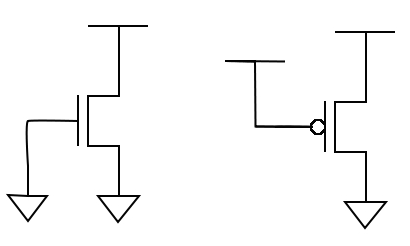
\includegraphics[width=0.4\textwidth]{img/mos_off.png}
\caption{Leakage drain/source current when MOS are off}
\label{fig:ds_leakage}
\end{center}
\end{figure}

\item $\mathbf{I_{GATE}}$ \textbf{- Gate Current}: is the leakage current that flows from drain and source to gate or vice versa when $|V_{GS}|=V_{DD}$ and $V_{DS}=0$  as can be seen in fig \ref{fig:gate_leakage}. Also in other condition a small gate current could appear but is possible to say that in those other cases the contribution is negligible.
\begin{figure}[htbp]
\begin{center}
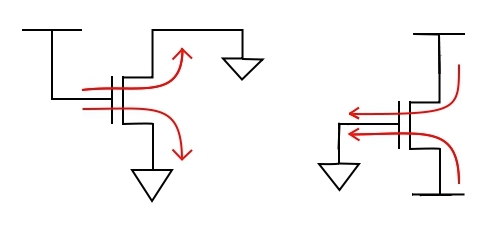
\includegraphics[width=0.4\textwidth]{img/mos_gate.jpg}
\caption{Leakage gate current}
\label{fig:gate_leakage}
\end{center}
\end{figure}

\end{itemize}

\subsection{Static power calculation}

As example the detailed procedure used to estimate the static power of the \textit{NAND2-CMOS} is presented.\\
Every possible combination of the two inputs are considered and for each of those cases the different appearing leakages contribution are taken into account.
The table \ref{tab:i_leakage_CMOS} is used to show this operation.
\begin{table}[htb]
\centering
\begin{tabular}{|c|c|c|c|}
\hline
A & B & Y & LEAKAGE CURRENT\\
\hline
0 & 0 & 1 & $ I_{OFFn} 2W_N+2\cdot I_{GATEp}W_P$\\
\hline
0 & 1 & 1 & $I_{OFFn}2W_N+ I_{GATEn}2W_N+I_{GATEp}W_P$\\
\hline
1 & 0 & 1 & $I_{OFFn}2W_N+I_{GATEp}W_P$\\
\hline
1 & 1 & 0 & $2\cdot I_{OFFp}W_P+2\cdot I_{GATEn}2W_N$\\
\hline
\end{tabular}
\caption{Leakage current contributes for each combination of inputs}
\label{tab:i_leakage_CMOS}
\end{table}\\
$I_{OFF}$ is the drain/source off current and $I_{GATE}$ is the gate current. Those contribution are multiplied by the effective dimension of transistor.\\
Considering the inputs as equally probable is possible to found the total leakage current as the mean value:
\begin{equation}
I_{leakCNAND2}=  {1 \over 4}\cdot(2 \cdot I_{OFFp}W_P+4 \cdot I_{GATEp}W_P+3 \cdot I_{OFFn}2W_N+3 \cdot I_{GATEn}2W_N) \quad [nA]
\end{equation}
Exploiting the same analysis is possible to found an expression for the static current for all the other gates.
Only the final expression are reported below.
\begin{itemize}
\item \textbf{NAND3-CMOS}:\\
 $I_{leakCNAND3} ={1 \over 8}\cdot(3 \cdot I_{OFFp}W_P+12 \cdot I_{GATEp}W_P+7 \cdot I_{OFFn}3W_N+7 \cdot I_{GATEn}3W_N) \quad [nA]$

\item \textbf{NAND4-CMOS}:\\
$I_{leakCNAND4}= {1 \over 16}\cdot(4 \cdot I_{OFFp}W_P+32 \cdot I_{GATEp}W_P+15 \cdot I_{OFFn}4W_N+15 \cdot I_{GATEn}4W_N) \quad [nA]$

\item \textbf{NOR2-CMOS}:\\
$I_{leakCNOR2}={1 \over 4}\cdot(3 \cdot I_{OFFp}2W_P+3 \cdot I_{GATEp}2W_P+2 \cdot I_{OFFn}W_N+4 \cdot I_{GATEn}W_N) \quad [nA]$

\item \textbf{NOR3-CMOS}:\\
$I_{leakCNOR3}= {1 \over 8}\cdot(7 \cdot I_{OFFp}3W_P+7 \cdot I_{GATEp}3W_P+3 \cdot I_{OFFn}W_N+12 \cdot I_{GATEn}W_N) \quad [nA]$

\item \textbf{NOR4-CMOS}:\\
$I_{leakCNOR4}={1 \over 16}\cdot(15 \cdot I_{OFFp}4W_P+15 \cdot I_{GATEp}4W_P+4 \cdot I_{OFFn}W_N+32 \cdot I_{GATEn}W_N) \quad [nA]$

\end{itemize}
\newpage


\section{Octave Implementation}

In table \ref{tab:input_dep} the variables  used  into the modules are reported and in table \ref{tab:output_var} there are the output parameters estimates.
\begin{table}[htbp]
	\begin{center}
		\begin{tabular}{|c|c|c|}
			\hline
			Code variable & Source file & Physical quantity\\
			\hline
			Lgate & Technology file & $nm$\\
			\hline
			Wgate & Technology file & $\mu m$\\
			\hline
			Vdd & Technology file & $V$\\
			\hline
			Xj & Technology file & $nm$\\
			\hline
			Cox & Technology file & $ F/ cm^2$\\
			\hline
			Cj0n & Technology file & $pF/\mu m^2$\\
			\hline
			Cjswn & Technology file & $pF/\mu m^2$\\
			\hline
			Cj0p & Technology file & $pF/\mu m^2$\\
			\hline
			Cjswp & Technology file & $pF/\mu m^2$\\
			\hline
			Cgd0n & Technology file & $F/m$\\
			\hline
			Cgd0p & Technology file & $F/m$\\
			\hline
			Gamma & Technology file & $-$\\
			\hline
			Mjn & Technology file & \% \\
			\hline
			Mjp & Technology file & \% \\
			\hline
			Mswn & Technology file & \% \\
			\hline
			Mswp & Technology file & \% \\
			\hline
			Pbn & Technology file & $V$ \\
			\hline
			Pbp & Technology file & $V$ \\
			\hline
			Pbswn & Technology file & $V$ \\
			\hline
			Pbswp & Technology file & $V$ \\
			\hline
			mueff\_n & Mobility module & $cm^2/Vs$\\
			\hline
			mueff\_p & Mobility module & $cm^2/Vs$\\
			\hline
			Vth\_n & Vth module & $V$\\
			\hline
			Vth\_p & Vth module & $V$\\
			\hline
			Ioff\_n & Ioff module & $\mu A/\mu m$\\
			\hline
			Ioff\_p & Ioff module & $\mu A/\mu m$\\
			\hline
			Igate\_n & Igate module & $\mu A/\mu m$\\
			\hline
			Igate\_p & Igate module & $\mu A/\mu m$\\
			\hline
		\end{tabular}
	\end{center}
	\caption{Variables required and used by the module}
	\label{tab:input_dep}
\end{table}
\begin{table}[htbp]
	\begin{center}
		\begin{tabular}{|c|c|c|}
			\hline
			Code variable & Physical quantity & Meaning\\
			\hline
			Delay\_nand\_and & $ns$ & input to output delay of selected module\\
			\hline
			Pnand\_and\_dyn & $W$ & Dynamic power of selected module\\
			\hline
			Pnand\_and  & $W$ & Static power of selected module\\
			\hline
		\end{tabular}
	\end{center}
	\caption{Variables provided in output of selected module}
	\label{tab:output_var}
\end{table}
\newpage
\subsection{Text Results}
An example of the output provided by the TAMTAMS analysis using the \textit{Print text results} is provided below.
The computed values of delay, dynamic and static power are reported for four possible value of \textit{Fan Out} where this quantity just means the number of inverter considered as output load for the gate.
\footnotesize
\begin{verbatim}

    Technology: bulk/HP_2005 

    System Setup: 2016-04-17 13:37:08 
    Cox =  2.8776e-06
    Vtlong =  0.61691
    SCE =  0.18990
    DIBL =  0.24118
    mueff_n =  252.01
    mueff_p =  61.319
    Ecrit_n =  7.9360e+04
    Ecrit_p =  3.2616e+05
    Vdsat_n =  0.15325
    Vdsat_p =  0.41401
    Cdep =  5.0656e-07
    m =  1.2831

    Module 0 : Delay_Pow_nand2_cmos 

    Fan Out = 1:
    I/ODelay[ns]  DynPower[W]  StaticPower[W]
     6.1742e+00   1.5764e-06   3.8419e-09

    Fan Out = 2:
    I/ODelay[ns]  DynPower[W]  StaticPower[W]
     9.6946e+00   1.8727e-06   3.8419e-09

    Fan Out = 3:
    I/ODelay[ns]  DynPower[W]  StaticPower[W]
     1.3215e+01   2.1691e-06   3.8419e-09

    Fan Out = 4:
    I/ODelay[ns]  DynPower[W]  StaticPower[W]
     1.6735e+01   2.4654e-06   3.8419e-09
\end{verbatim}
\normalsize
\subsection{Graphical Results}
Using the  \textit{Show graphical results} three different graph are provided as output. The first one represents the delay; an example is reported in fig. \ref{fig:delay_out}. There are four different lines, one for each value of \textit{Fan Out}. \\
The figure \ref{fig:dpower_out} shows the second graph provided and it represent the dynamic power.\\ The last graph shows the static power (fig. \ref{fig:spower_out}). This value does not depends on output load so all the lines are overlapped.\\
\begin{figure}[htbp]
	\begin{center}
		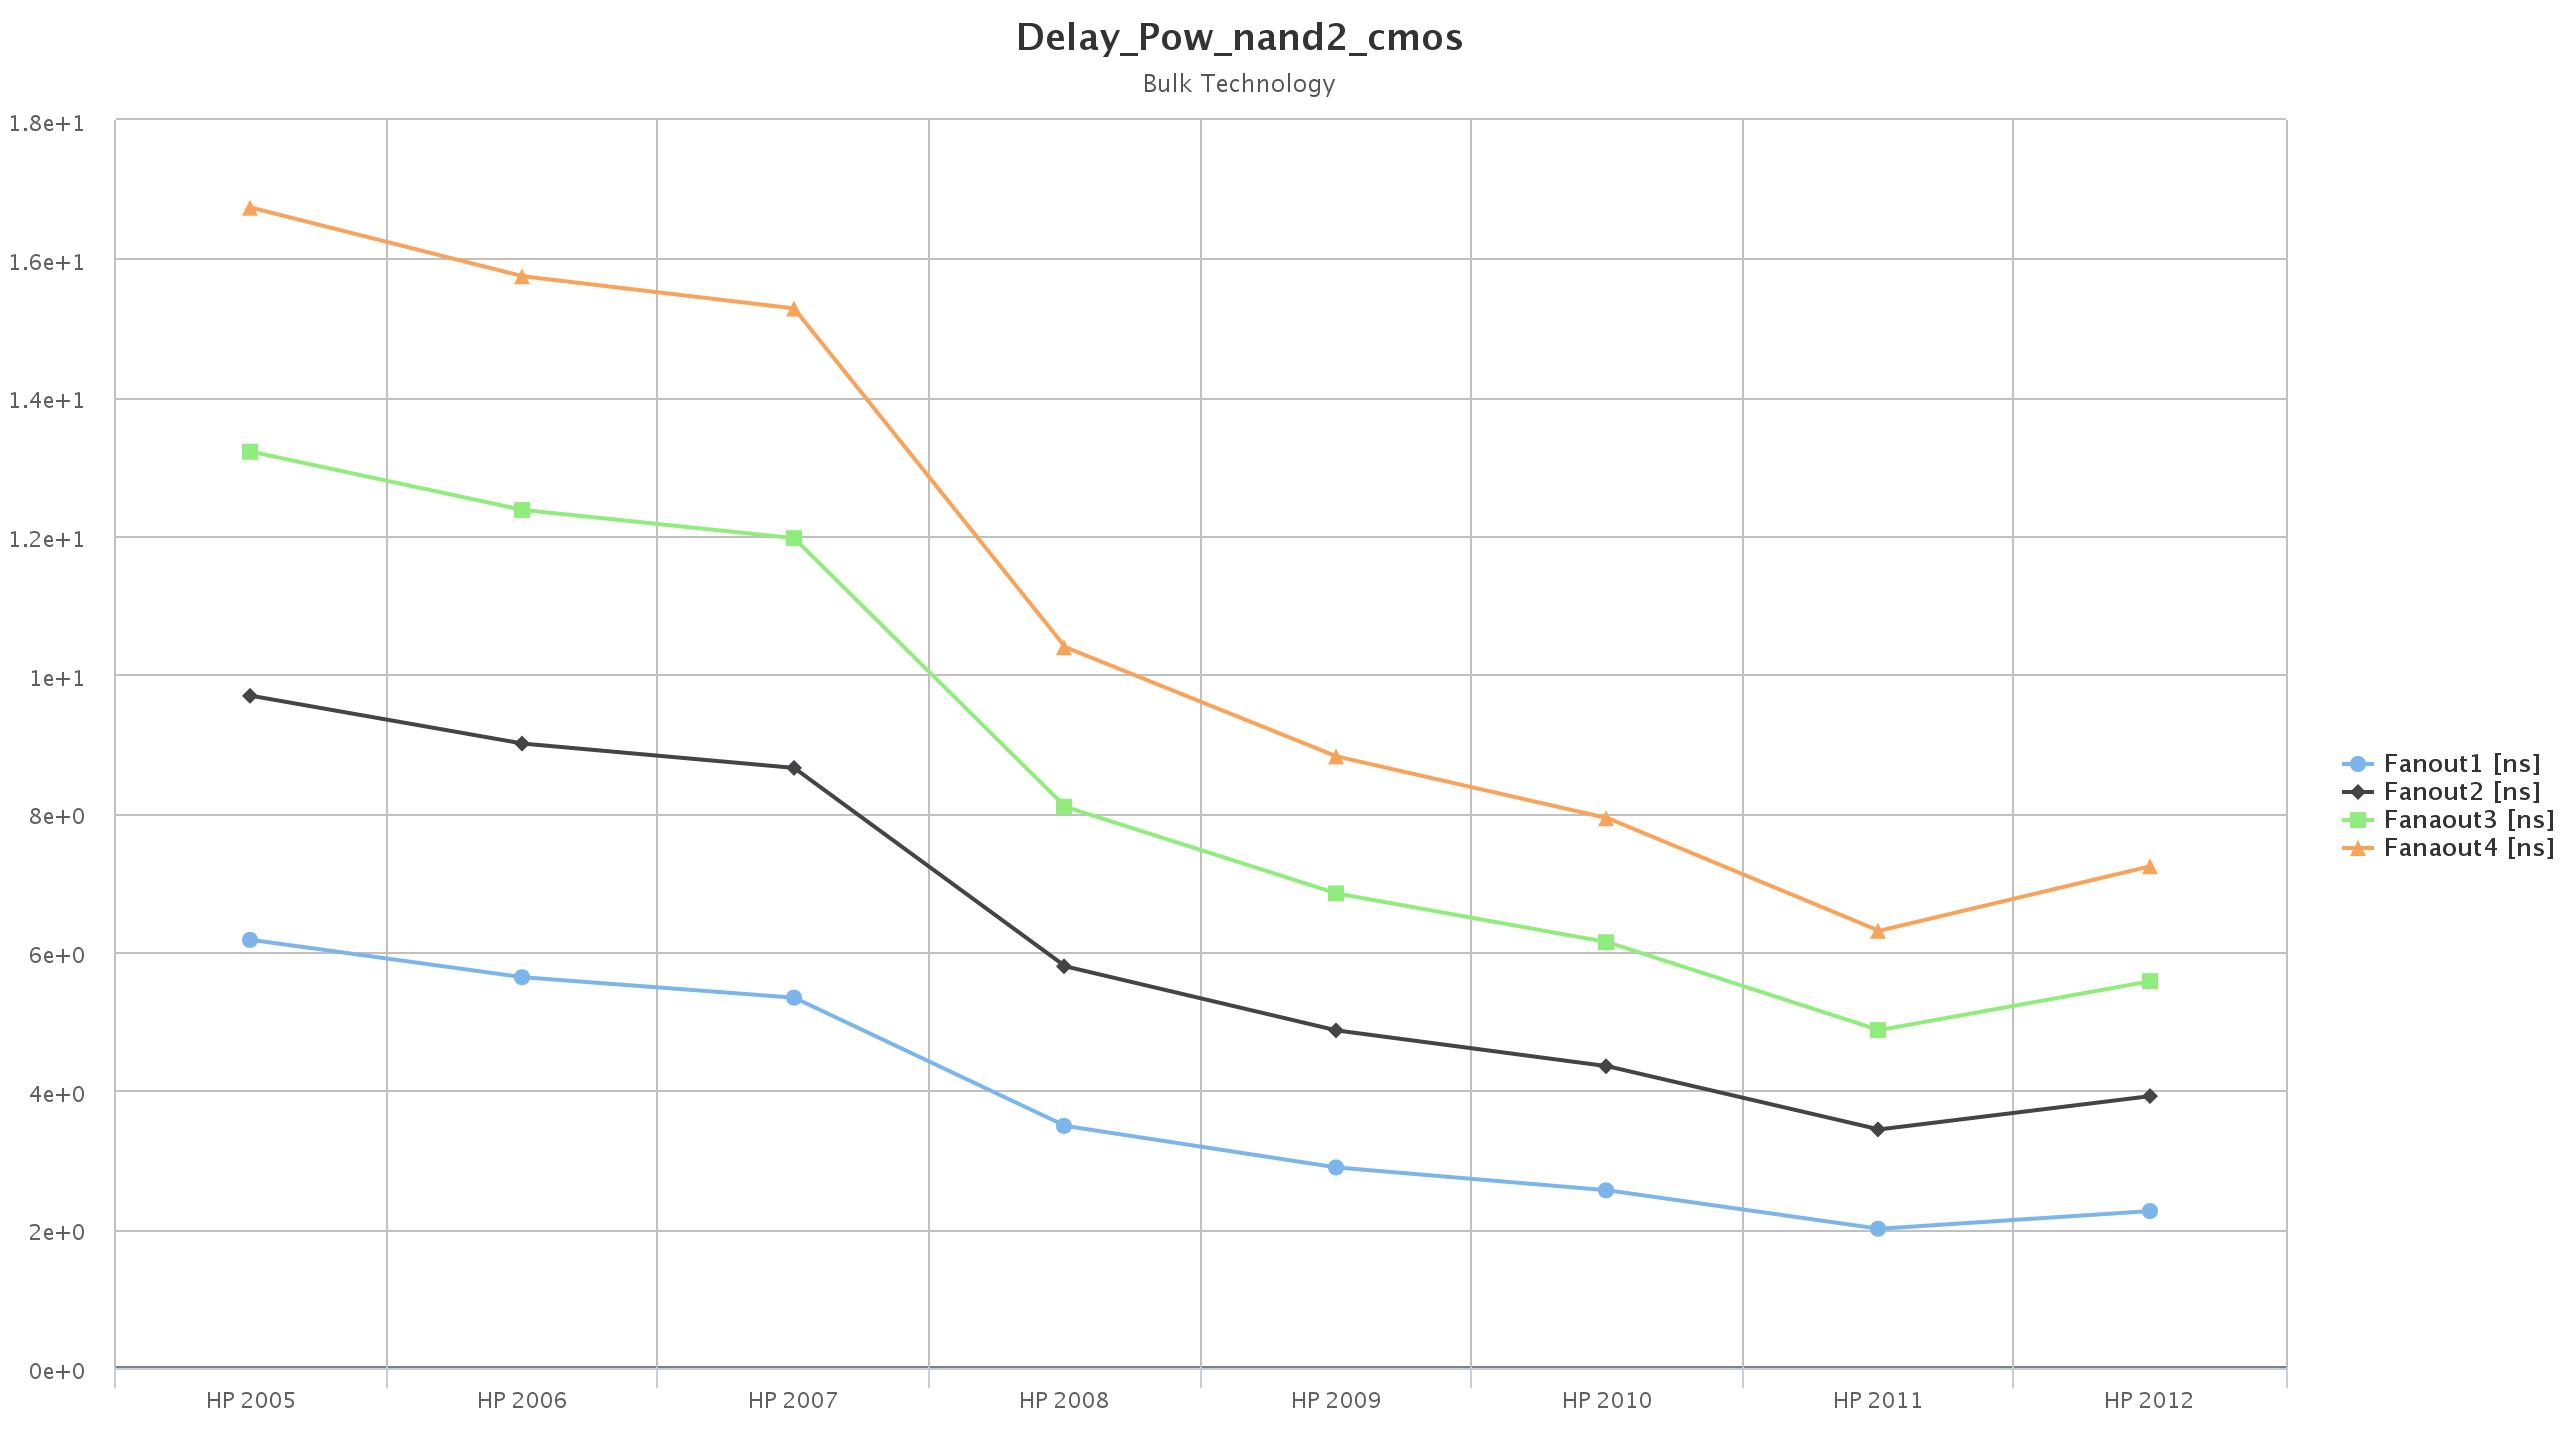
\includegraphics[width=17cm]{img/Delay_Pow_nand2_cmos_Delay.jpeg}
		\caption{Delay graphical output}
		\label{fig:delay_out}
	\end{center}
\end{figure}

\begin{figure}[htbp]
	\begin{center}
		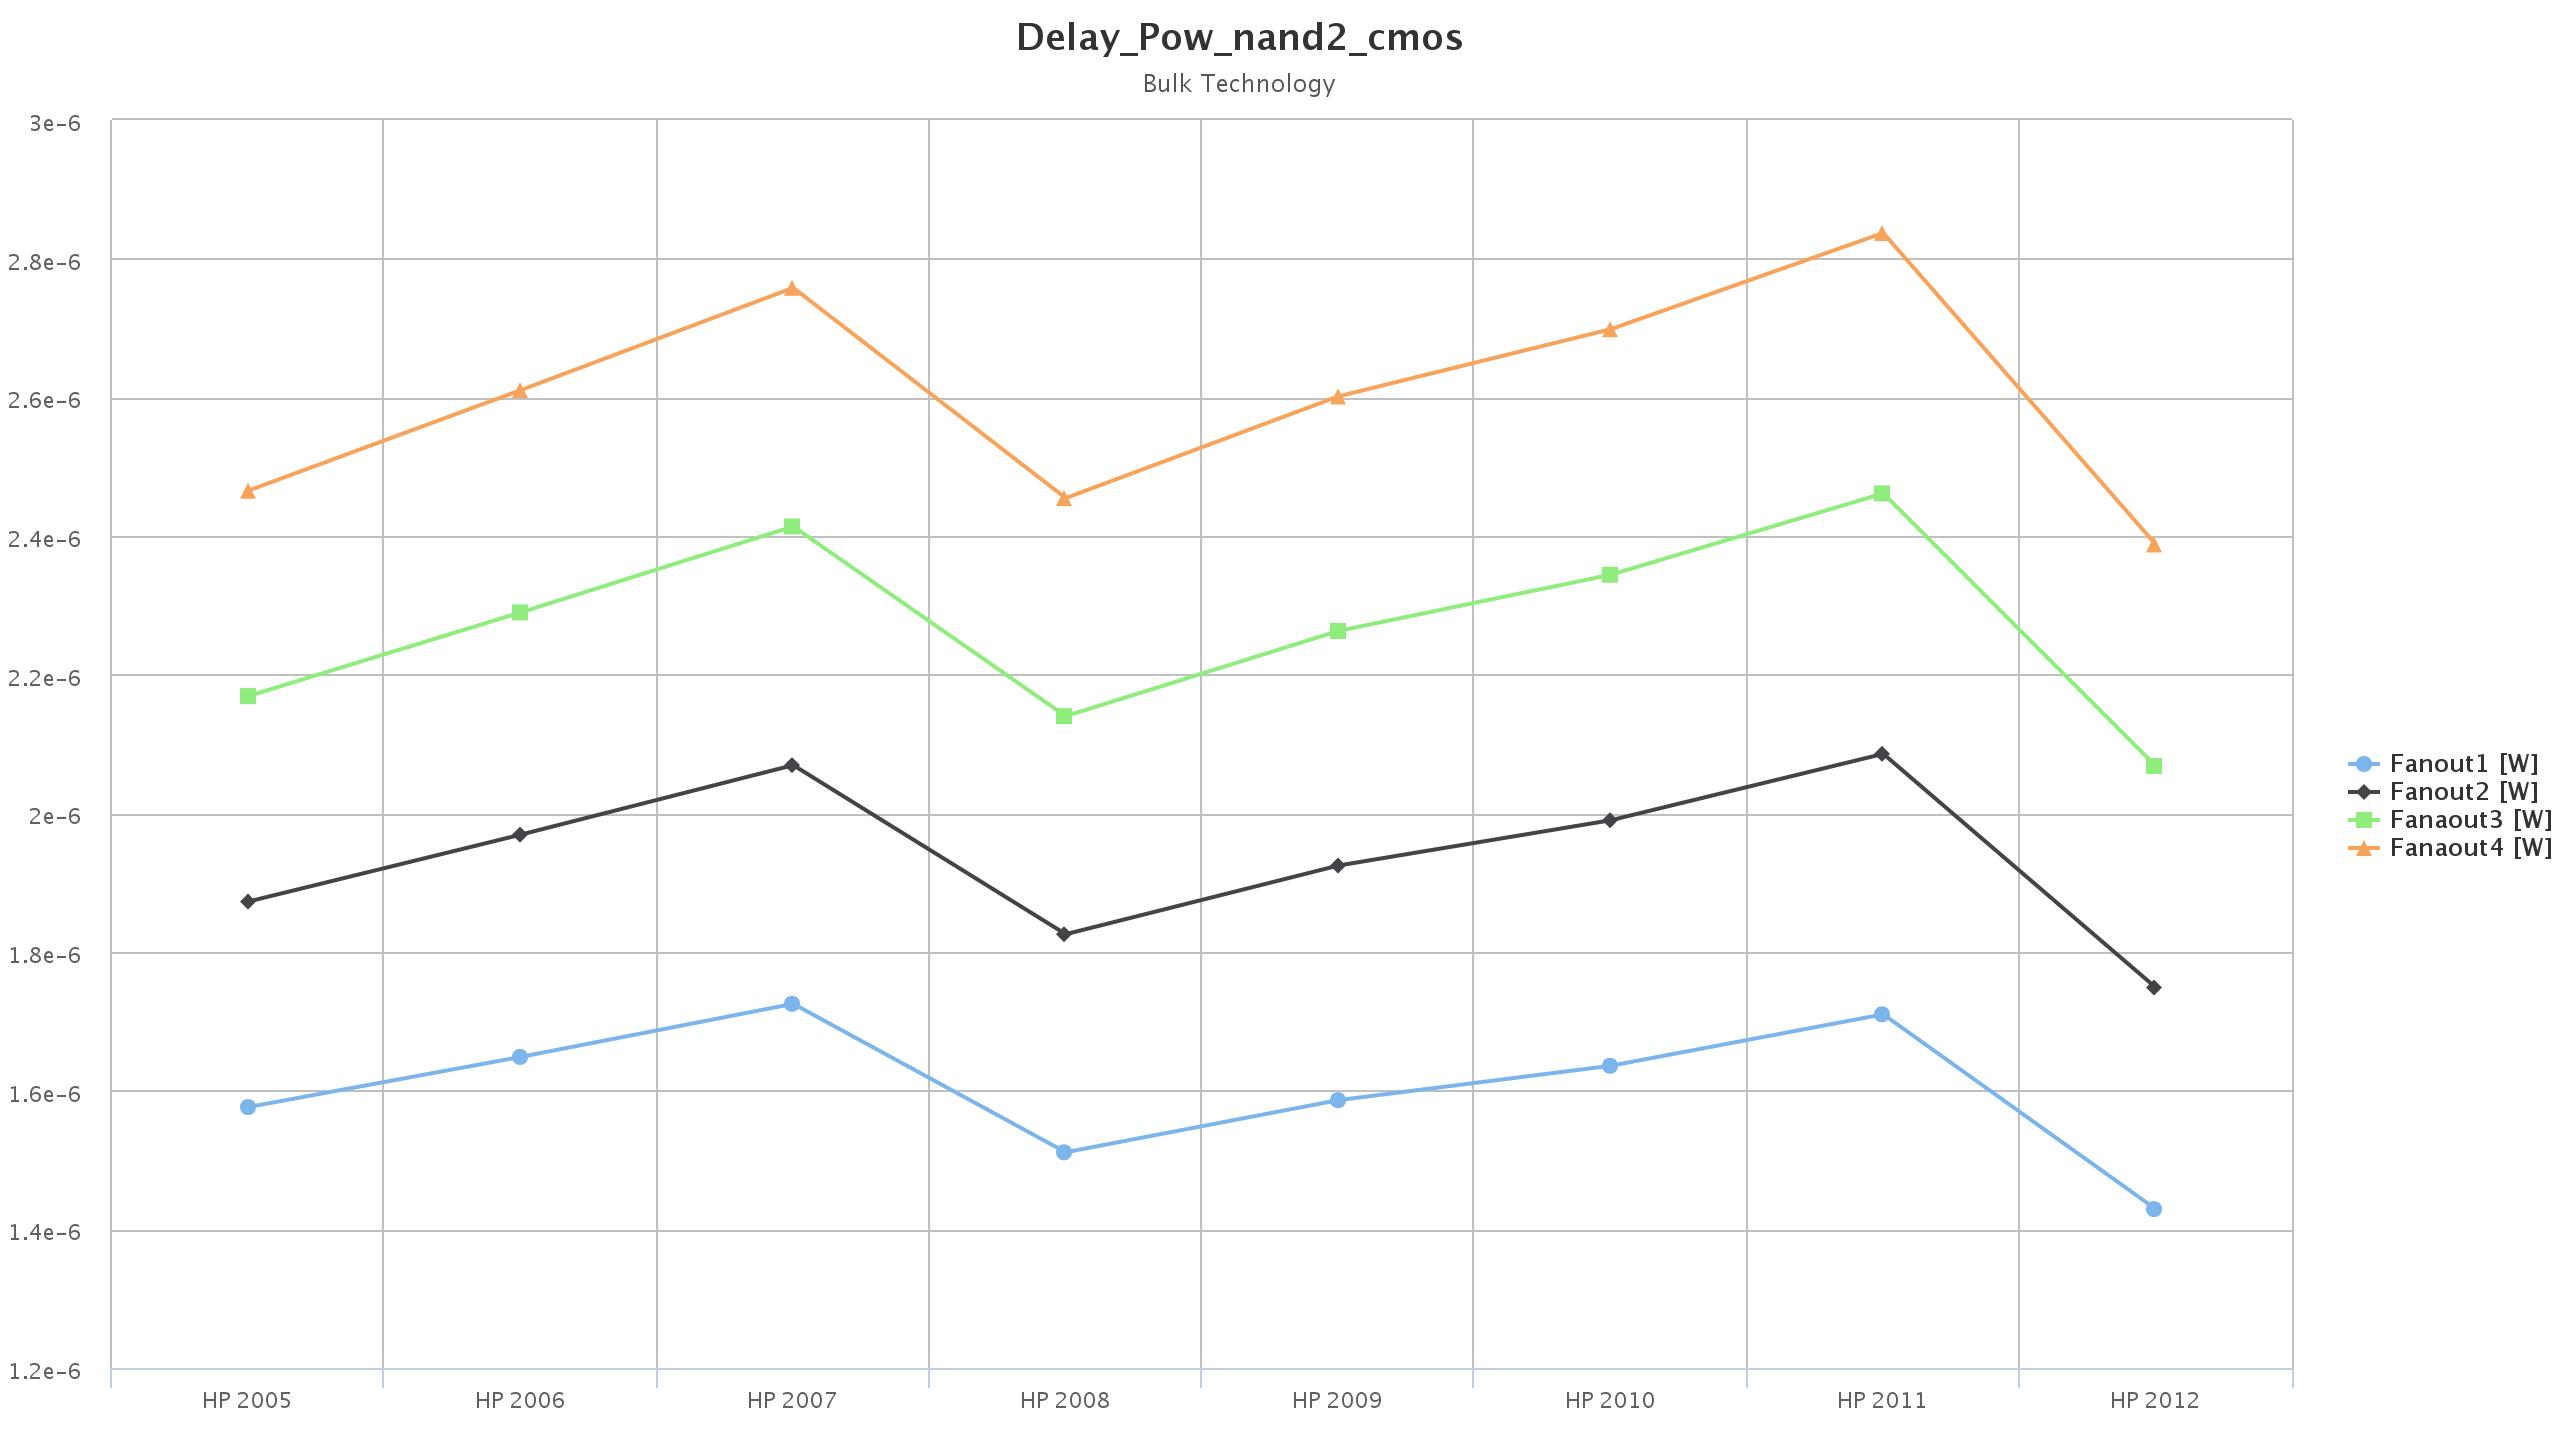
\includegraphics[width=17cm]{img/Delay_Pow_nand2_cmos_Dpower.jpeg}
		\caption{Dynamic power graphical output}
		\label{fig:dpower_out}
	\end{center}
\end{figure}

\begin{figure}[htbp]
	\begin{center}
		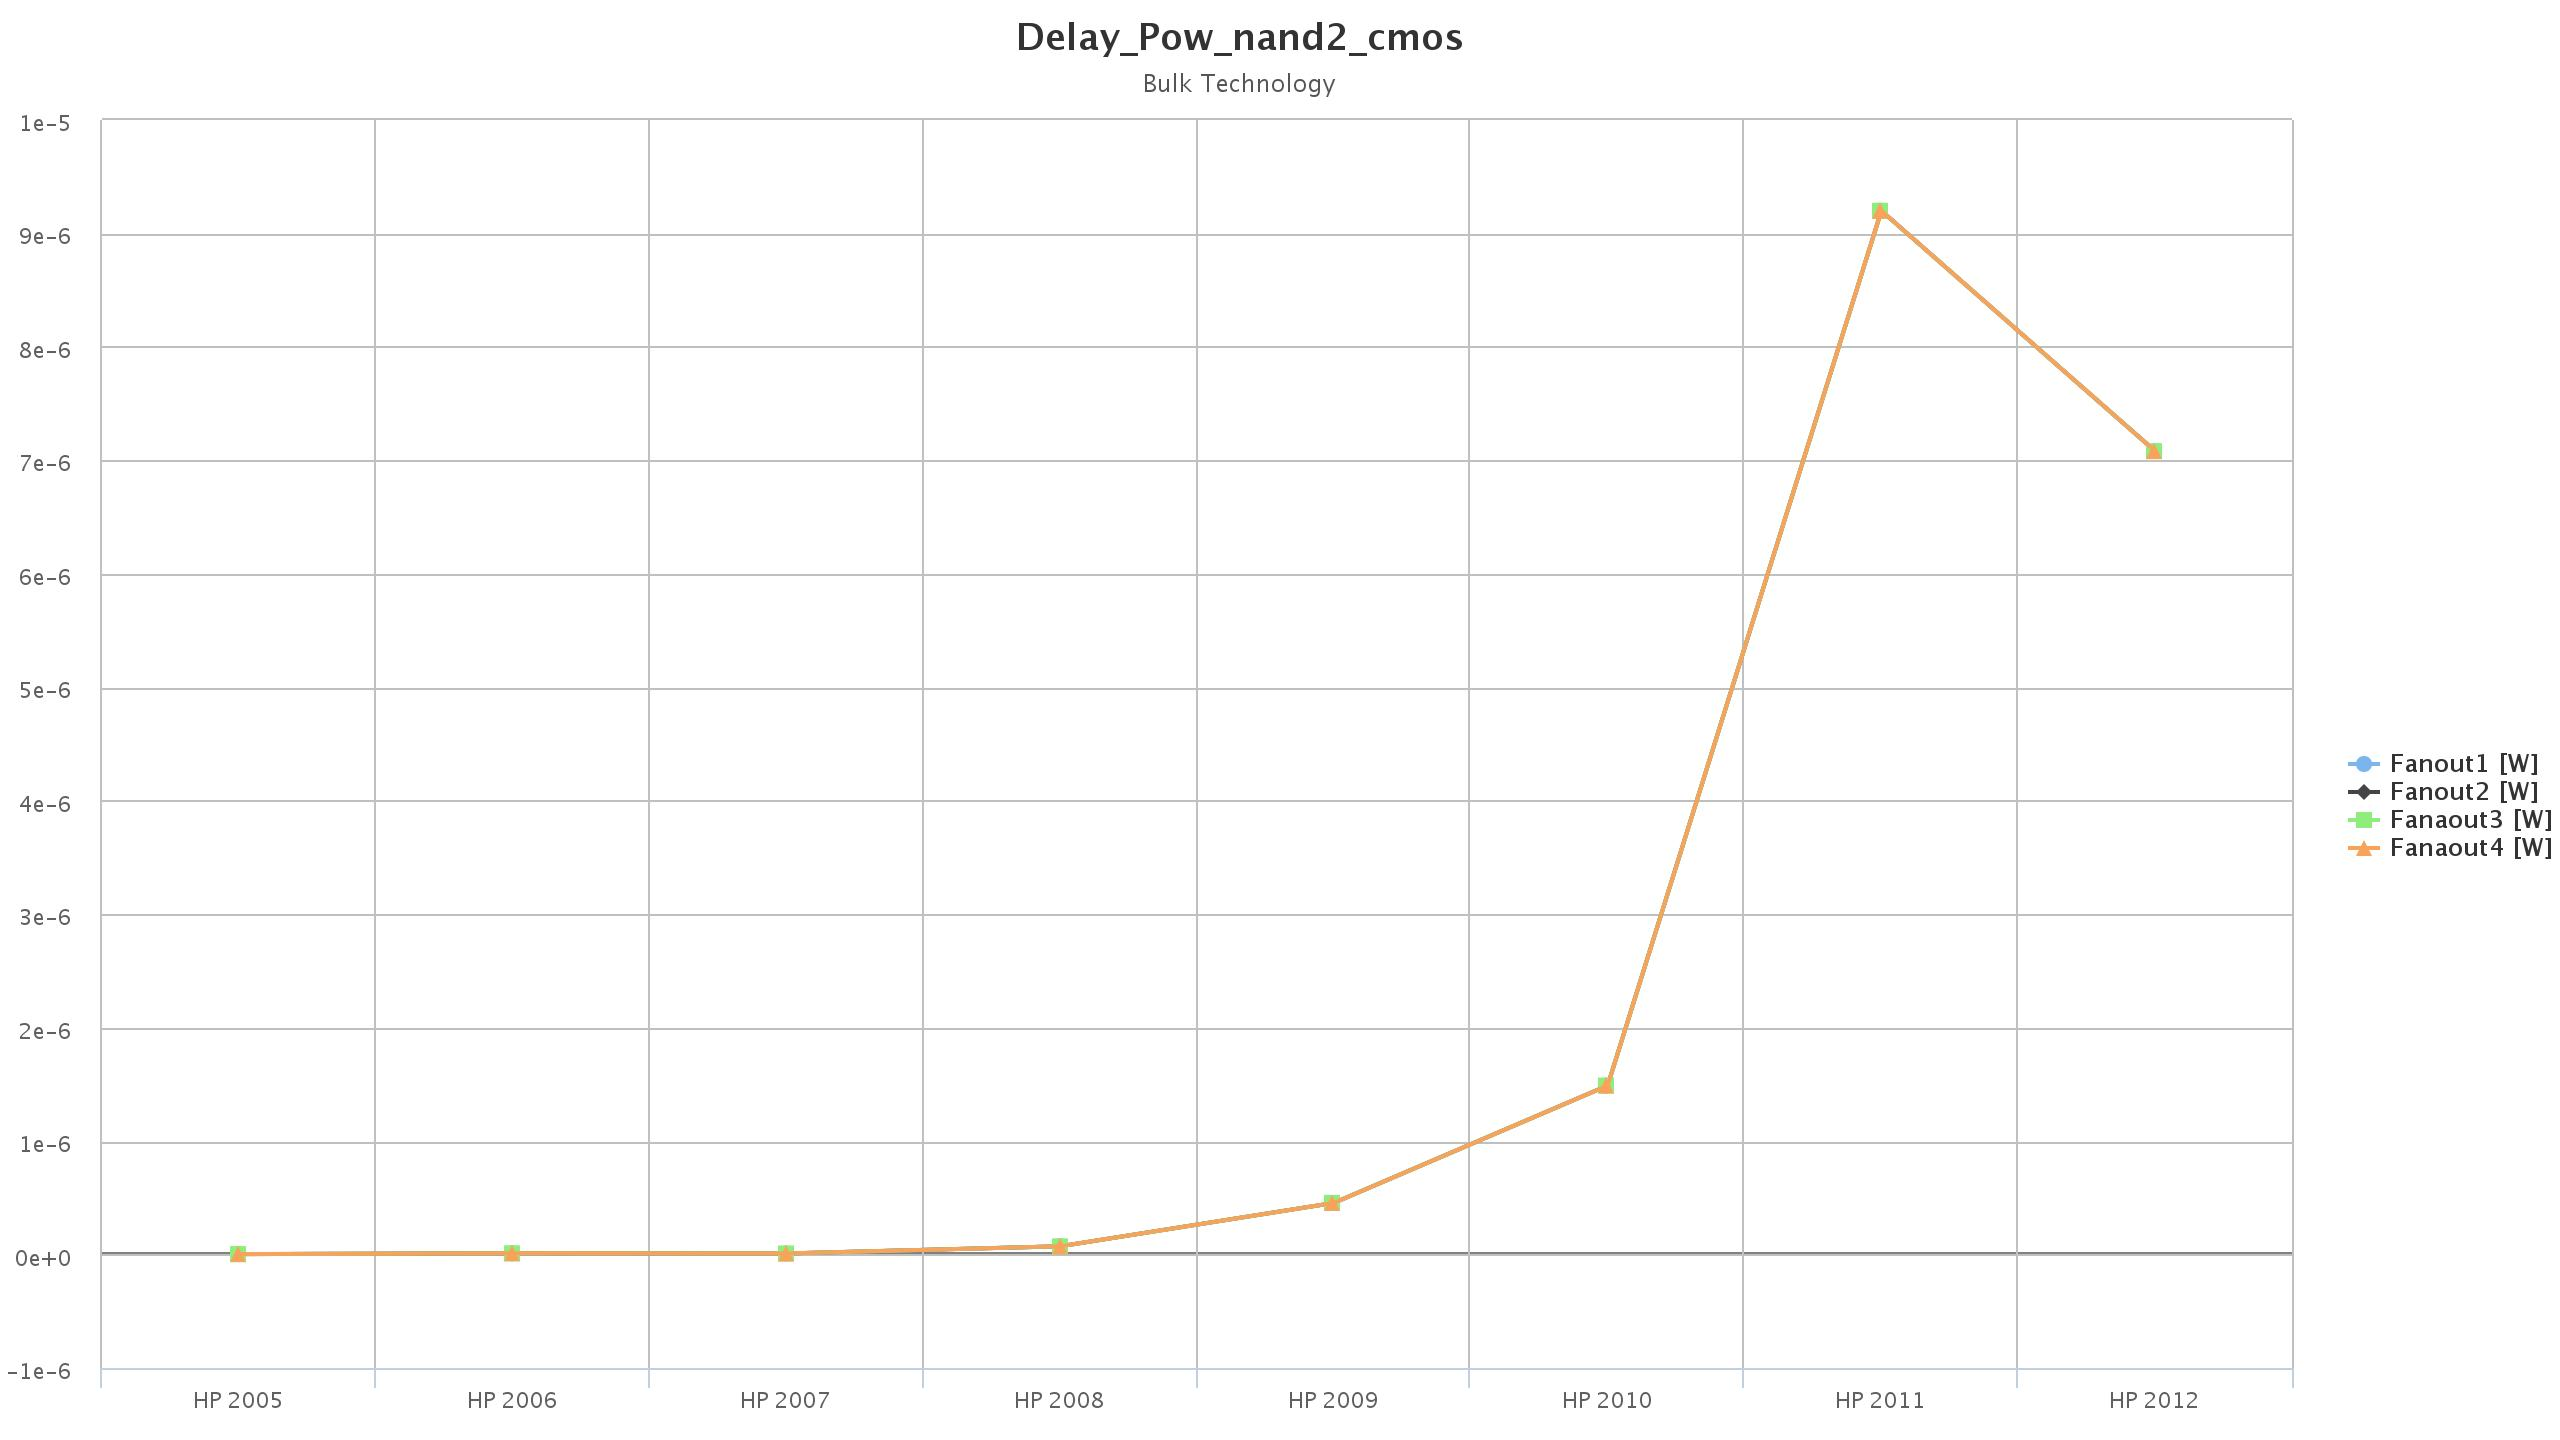
\includegraphics[width=17cm]{img/Delay_Pow_nand2_cmos_Spower.jpeg}
		\caption{Static power graphical output}
		\label{fig:spower_out}
	\end{center}
\end{figure}

\end{document}

